\section{A stochastic model for finite Knudsen numbers}
Toschi and Succi~\cite{Toschi2005} have proposed a stochastic model that
works well for intermediate Knudsen numbers, as verified for a long microchannel. 
In their article, they focus on the problem
that appears when trying to map a continuous direction space to a finite set of
directions. In particular, they note that molecules that were going to travel in
a direction slightly different than the (parallel to the lattice) flow direction,
and collide with the wall after some time, are actually mapped to a direction
in which they will never take part in a collision with the solid boundaries.
This case is shown in figure~\ref{fig:Toschi}. 

\begin{figure}[h!]%
 	\begin{center}%
 		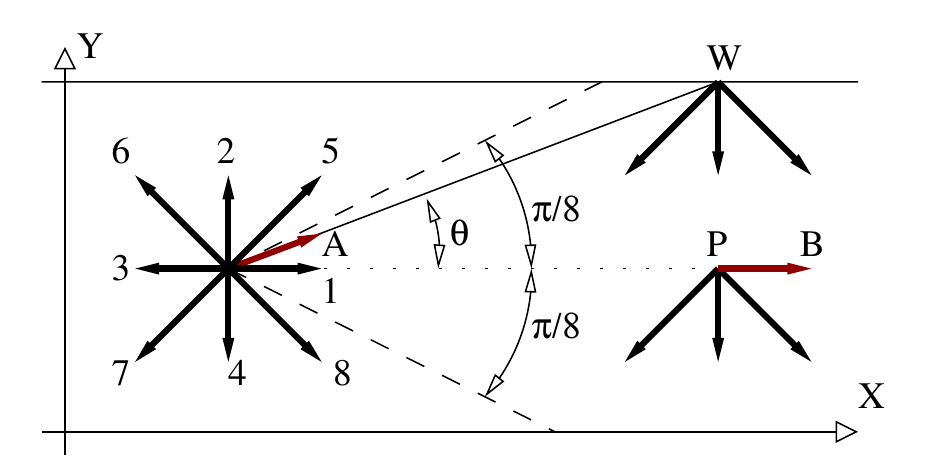
\includegraphics[scale=0.35]{Toschi}%
 		\caption{All the molecules that were going to travel within the %
 		$-\pi/8 < \theta < \pi/8$ range are actually mapped to %
 		a single direction. Because this direction is parallel to the flow, %
 		and because the intermolecular collisions are rare, these molecules %
 		will never collide with the walls and they will continue accelerating.~\cite{Toschi2005}}%
 		\label{fig:Toschi}%
 	\end{center}%
\end{figure}

Because of the external forcing (i.e.\@ a pressure gradient), an accelerating beam
is created. Remember that, in high Knudsen number regions, the particles relax their
properties mainly by interacting with the wall. 
To solve this problem, Toschi and Succi introduce a probability distribution
for the direction after the collision, they use a virtual-wall-collision mechanism and they
try the normal bounce-back and the Ansumali-Karlin boundary conditions.
The latter ones re-inject molecules from the wall, in order to maintain the
local equilibrium in respect to wall speed and temperature.

In order to model \textit{virtual wall collisions}, they assign a \textit{virtual speed A}
$(u_\mathrm{x}, u_\mathrm{y}) = c \cdot (\cos \theta, \sin \theta)$ with $\theta$
uniformly distributed in $[-\pi/8 , \pi/8]$ and they assume that the collisions
follow a Poisson distribution. In this context, they define the probability
of virtual wall collision as the probability to skip intermolecular collisions before hitting
the wall, multiplied by the probability to collide with the wall in a time step:
\begin{equation}
 p(x, y; t) = \exp( -1/\mathrm{Kn} ) \cdot \Big( 1 - \exp \Big( - \frac{c \cdot \mathrm{d}t \cdot \sin(\theta(x,y))}{H} \Big)   \Big)
\end{equation}
This probability vanishes for very small Knudsen numbers (continuum regime)
or for very small angles (direction parallel to the flow).

After colliding with e.g.\@ the upper boundary (as in fig.\,\ref{fig:Toschi}),
the particle distribution functions become:
\begin{eqnarray*}
 f'_1 = f_1(1-p) &\textrm{, \ \ } f'_{7,8} = f_{7,8} + p f_1 / 6 &\textrm{, \ \ } f'_4 = f_4 + 4 p f_1 / 6 \\
 f'_3 = f_3(1-p) &\textrm{, \ \ } f'_{5,6} = f_{5,6} + p f_3 / 6 &\textrm{, \ \ } f'_2 = f_2 + 4 p f_3 / 6
\end{eqnarray*}
where $\{ 1/6, 4/6, 1/6 \}$ correspond to the weights of the nine-speed lattice scheme.
Notice the different signs between the functions 1,3 and the other PDFs. With this formulation,
momentum is re-distributed from the directions parallel to the walls to the other directions.
This allows the system to relax towards a (non-local) equilibrium even for higher Knudsen numbers.

The authors test their model with Single-Relaxation-Time collision and apply both bounce-back
and Ansumali-Karlin boundary conditions for Knudsen numbers up to 30 and for Mach number 0.03.
They observe a minimum in mass flow at $\mathrm{Kn}\approx 1$, something that is physical
and is referred to as \textit{``Knudsen paradox''}, but both BC overestimate this minimum.
In general, the authors receive better results with Ansumali-Karlin boundary conditions,
in accordance with prior predictions, especially in lower-Knudsen regions.
